\documentclass{article}

% Includes preamble from standard file
% ==========================================================
%   GPR-20 MANUALS PREAMBLE
% ==========================================================

% ==========================================================
% Includes packages
\usepackage{array}
\usepackage{float}
\usepackage{parskip}
\usepackage{caption}
\usepackage{tabularx}
\usepackage{titlesec}
\usepackage{hyperref}
\usepackage{setspace}
\usepackage{graphicx}
\usepackage{listings}
\usepackage{xltabular}
\usepackage{csvsimple}
\usepackage{longtable}
\usepackage{subcaption}
\usepackage{indentfirst}
\usepackage[utf8]{inputenc}
\usepackage[margin=1in]{geometry}
\usepackage[type={CC}, modifier={by-nc}, version={4.0}]{doclicense}
\usepackage{subfiles}
% ==========================================================

% ==========================================================
% PREAMBLE SETTINGS
% Sets double spacing
\doublespacing

% Sets paragraph indentation
\setlength{\parindent}{1em}

% Sets paragraph skip
\setlength{\parskip}{2em}

\renewcommand{\arraystretch}{1.25}
% ==========================================================


% Adds bibliography
\usepackage[style=numeric]{biblatex}
\bibliography{biblio.bib}


% Defines command to insert name
\newcommand{\GPRManualName}{Software Guide}

% ==========================================================
% DOCUMENT INFORMATION
\title{GPR-20: Software Guide}
\author{Grupo de Desminado Humanitario}
\date{March 2021}
% ==========================================================

\begin{document}

\subfile{front}

\newpage
\section{Introduction}
The GPR-20 robot requires a complete software suite in order to acquire data and move to different coordinates within the sampling area. The robot acquires data from the subsurface using a Ground Penetrating Radar (GPR). The GPR consists of a Vector Network Analyzer (VNA) and two antennae. The GPR is moved within the sampling area using stepper motors. The actions of both acquiring data and moving the GPR are executed using commands from the robot software suite. The robot also requires an interface for the users to command it.

When operating, the robot will execute a survey: sampling the ground on different coordinates. There are three coordinates that are considered: X coordinate, Y coordinate and Z rotation. The X and Y coordinates refer to the location of the GPR in each axis. On the other hand, the Z rotation refer to the rotation of the antennae. This rotation is included to sample different electromagnetic polarizations. The acquired data is saved on a persistent storage when each point is sampled. Additional operations carried out during a survey consists of providing feedback to the user and acquiring the height from the antennae to the ground. The height is acquired from an infrared (IR) sensor located in the GPR.

The software suite is responsible of executing the commands required to perform the aforementioned actions. Many approaches can be used to develop the software in which one stands out: a software suite based on the Robotic Operating System (ROS). ROS is an open-source framework that provides libraries and tools to develop robotic applications. Using ROS to develop the software allowed to have modular packages that are then integrated into a graph-like architecture. Each package is part of a peer-to-peer network of processes that are loosely coupled using the ROS communication infrastructure. A detailed explanation of the ROS framework is addressed in this document.

Each of the GPR-20 actions has different requirements that constrain the device in which the software must be executed. Some actions such as acquiring and storing the VNA data require a considerable amount of computing power. Other actions require driving physical signals within a defined timing constrains. These requirements led to distributing the software on two devices: a Raspberry Pi 4 single-board computer and a personal computer. The Raspberry Pi 4 is used as the on-board computer i.e. it is physically located in the robot while the personal computer is connected to the robot via a network interface.

This document presents the GPR-20 software suite. It addresses a detailed explanation of the software execution environment, the software suite architecture, and a detailed explanation of each of the software packages. The document is organized as follows: first, it explains the used operating system. Then, the ROS framework is introduced in detail. The third section of the documents corresponds to a general overview on the software architecture. Each of the software packages is presented on the fourth section. Finally, a section is devoted to keep a record on how to extend and improve the software suite. 

\newpage
\section{Operating System: Canonical Ubuntu}
The operating system (OS) in which the GPR-20 software runs is Canonical Ubuntu (\href{https://ubuntu.com/}{link}). Ubuntu is a Debian-based Linux distribution that is developed and maintained by Canonical. It is one of the most popular Linux distributions and it is currently used on personal computers, servers and internet-of-things (IoT) devices. Releases for Ubuntu occurs every six months with long-term support releases happening every two years. Because of its popularity, Ubuntu provides support and easy-to-install mechanisms for different libraries and utilities. Within the context of the GPR-20 robot, this means that it simplifies the management of the required libraries and framework thus improving the development process.

The OS is used on both the on-board computer and the personal computer. The installation on the personal computer is straightforward and does not require to customize the operative system to fit any constrain. This is not the case for the Raspberry Pi 4. The on-board computer requires the operating system to minimize the RAM usage, CPU usage, and disk usage. This is addressed by tailoring Ubuntu to fit those requirements. The first requirement is the architecture of the Raspberry Pi BCM58712 SoC: ARMv8-A. Using a different architecture from x86 might arise compatibility issues on the OS itself and the libraries. However, Ubuntu is available on ARMv8-A and most of its libraries work on both architectures. In order to prevent issues from compatibility, each library is checked to ensure that it works on ARMv8-A.

Another requirement that must be addressed is disk space. The OS should minimize the disk usage since the main storage of the Raspberry Pi is a 16GB SD card. In order to minimize disk usage, the server version of  Ubuntu is used. The server version of Ubuntu does not include third-party software that is included in the desktop version of the OS thus reducing disk space usage. Using the server version also implies that no desktop environment is installed. A minimal desktop is installed since it is required to display the user interface of the robot. The installed desktop environment is Ubuntu MATE.

To ensure that the Raspberry Pi resources are used at their best, the Ubuntu 20.04 LTS version is used. It must be noted that the 18.04 LTS version was tested on the Raspberry Pi 4 but performance of the 20.04 LTS version was better. It also must be noted that Ubuntu is not the official OS for the Raspberry Pi but it was used since it simplifies the software development and improves compatibility with the personal computer as it runs Ubuntu. 

\newpage
\section{Framework: Robotic Operating System}
The main used framework is the Robotic Operating System (ROS, \href{https://ros.org/}{link}). Contrary to what its name suggest, the framework is not an operating system but a set of tools and libraries to develop robotic applications. ROS software is organized in \textit{packages}. Packages are the most atomic build and release item from ROS i.e. it is the most granular element that can be built and released. Packages contain ROS run-time processes that are defined as \textit{nodes} under ROS terminology. Nodes are the elements that perform computation thus providing the required capabilities from software. A package can contain multiple nodes depending on the application needs.

Besides from organizing the software, ROS also defines concepts for communication among nodes. The basic element for ROS communication are \textit{messages}. Messages are data structures that define typed fields. The data types that can be used depend on primitives that include numeric, Boolean, string and time types. The primitives can be arranged as arrays and nested structures if necessary. A message is defined in a \textit{msg} file and may contain an arbitrary amount of data fields.

The most simple communication mechanism provided by ROS consists of \textit{topics}. Topics are a transport system with a name and a message type in which any node can \textit{publish} or \textit{subscribe}. Publishing is the act of a topic sending out a message through the topic. On the other hand, subscribing refers to a topic retrieving data from the topic. Another communication mechanism provided by ROS are \textit{services}. Services provide a request/reply communication between two agents. A service is defined by two messages that have the request and reply definition in a \textit{.service} file. Services are similar to remote procedure calls and are blocking: the sender must wait until receiving the response.

A third communication mechanism are \textit{actions}. Actions are not a primitive communication mechanism but an extension to ROS. Actions are similar to services in the sense that they provide a request/reply communication. Actions differ from services as they provide support for non-blocking calls. In other words, actions do not require the sender to wait for the reply as services do. An action is specified by three messages: \textit{goal}, \textit{feedback} and \textit{result}. The goal defines the input data required to execute the procedure. The feedback is used to provide the sender with the progress of a goal. Finally, the result defines the output data of the procedure. The three required messages of an action are defined in a single \textit{.action} file.

Applications using ROS can be represented as graph. Nodes in the graph are the processes i.e. the ROS nodes in which computation takes place. The graph edges are the communication mechanisms provided by ROS: topics, services and actions. This architecture provide benefits for robotics applications such as decoupling the processes to build complex systems. On the other hand, the decoupled processes have a more specific purpose thus facilitating its development. In general terms, a robotic application can be developed easily when using ROS, and this is the reason behind ROS popularity among the robot community.

\newpage
\section{Software Architecture Overview}
The software suite for the GPR-20 robot is developed under the ROS framework thus generating a graph-like architecture. Nevertheless, the graph is not enough to describe the architecture. Specific details of each element must be addressed in order to correctly describe and justify the architecture. This section is devoted to describe the requirements of the software suite and how it is organized to fulfill them. First, the general requirements of the software are specified. Then, the requirements are linked to a ROS package and organized in a graph architecture. Finally, implementation details are addressed.

\subsection{General Requirements}
The GPR-20 robot purpose is to acquire Ground Penetrating Radar (GPR) data from deactivated minefields. In order to acquire the data, the robot must be able to get the data from a Vector Network Analyzer (VNA) and save it in a persistent storage. The VNA and the antennae must be moved within a sampling area to effectively acquire relevant data. The height between a fixed point of the antennae and the ground is also acquired and stored. Finally, an user interface must be provided in order to define the data-acquisition parameters. A summary of the global requirements for the GPR-20 software suite is presented on table \ref{tab:software_requirements}.

\begin{table}[h]
    \centering
    \begin{tabular}{|c|p{10cm}|}
         \hline \multicolumn{1}{|c|}{\textbf{Number}} & \multicolumn{1}{c|}{\textbf{Requirement}} \\ \hline
         1 & Communicate with the VNA to acquire data. \\ \hline
         2 & Save the VNA data in a persistent storage. \\ \hline
         3 & Move the GPR within the sampling area \\ \hline
         4 & Acquiring height data. \\ \hline
         5 & Save height data in a persistent storage. \\ \hline
         6 & Provide an user interface to set the data-acquisition parameters. \\ \hline
    \end{tabular}
    \caption{Global requirements for the GPR-20 software suite.}
    \label{tab:software_requirements}
\end{table}

Table \ref{tab:software_requirements} presents a summary of the software requirements and associates them with a number. Requirement number one (1) defines that data must be retrieved from the VNA. In order to communicate with the VNA, the software can make use of the VXI-11 protocol. The VXI-11 protocol is supported by the VNA and since it relies on the TCP/IP protocol, it only requires a network interface. The user manual of the VNA defines the messages to configure the device and retrieve the data. 

Saving data is specified in requirements two (2) and five (5) in which respectively, VNA and height data is saved in persistent storage. Going beyond the definition of persistent storage, two options arise: storage devices and cloud storage. However, since the robot might operate in a place in which no Internet is available, cloud storage is discarded as a first-hand approach. Cloud storage may be used as backup and/or to share the data with the community. Storage devices include hard-drive drives (HDDs), solid-state drives (SSDs), SD cards and USB flash drives. Since the software will execute on either a personal computer (HDD and/or SSD) or the Raspberry Pi 4 (SD card), data will be stored in one of those devices. Since acquired data size can be in the order of gigabytes (GBs), either the HDDs or the SSDs will be preferred.

Requirement number three (3) indicates that the GPR will move within a sampling area. The movement of the GPR is handled using five stepper motors: three for moving along the X and Y axes and two for rotating the antennae. The motors are controlled using \textit{drivers}, that in turn are controlled using a two-signal protocol. The protocol signals are required to have specific timing requirements in order for the motors to work. These signals are intended to be driven from the Raspberry Pi 4 single-board computer. Endstop sensors are used in each axis as a way to tell the position of an axis on startup.

Requirement number four (4) states that height data must be also acquired. The height data is acquired using an infrared (IR) sensor located in the GPR mount. The IR sensor output is a signal in which its voltage corresponds to a specific height. Since neither the Raspberry Pi 4 or the personal computer has an analog/digital converter (ADC), an external one is required. The ADC communicates using the SPI protocol thus the Raspberry Pi 4 is the best option to acquire the data.

Finally, requirement number six (6) indicates that an user interface should be provided. An user interface can be a command-line interface (CLI) or a graphical user interface (GUI). Since using a CLI requires the user to know how to use a command line in first place, it is discarded in favor of a GUI. The GUI should be designed for an inexperienced user to interact with the robot.

\subsection{Architecture Definition}
A software architecture can be defined keeping into account the requirements from table \ref{tab:software_requirements}. The first defined set of elements are the processing elements of the architecture i.e. the ROS nodes. The ROS nodes are defined based on the general software requirements and constrains generated by the implementation itself. Table \ref{tab:software_nodes} presents the processing nodes that will be used in the architecture with a brief description of their purpose.

\begin{table}[h]
    \centering
    \begin{tabular}{|l|p{10cm}|}
        \hline  \multicolumn{1}{|c|}{\textbf{Name}} & \multicolumn{1}{c|}{\textbf{Purpose}} \\ \hline
        Axis Driver & Handles the movement of a single axis of the robot. \\ \hline
        Height Sensor & Samples data from the height sensor ADC through the SPI protocol. \\ \hline
        VNA Acquisition & Manages the communication with the VNA device. It can configure and retrieve data from the device. \\ \hline
        Data Processing & Stores the VNA and height sensor data in a persistent storage. \\ \hline
        User Interface & Provides a graphical user interface from which the user can interact with the robot. \\ \hline
        Main Control & Provides synchronization mechanisms within the robot software. \\ \hline
    \end{tabular}
    \caption{Defined nodes for the GPR-20 software suite.}
    \label{tab:software_nodes}
\end{table}

The \texttt{Axis Driver} node aims to fulfill requirement number three (3) by handling the axes movement. The \texttt{Axis Driver} node must be able to manage the movement of linear and rotational axes. Depending on the movement type, the node should sample the endstop sensor. The same \texttt{AxisDriver} node must be used for the three axes. The \texttt{Height Sensor} node fulfills requirement number four (4). It retrieves data from the ADC using the SPI protocol. The node must retrieve data from the ADC and then calculate its distance value. The \texttt{VNA Acquisition} node fulfills requirement number one (1). It is able to configure the device and acquire data via the VXI-11 protocol. The \texttt{Data Processing} node fulfills requirement number two (2) and five (5). The node processes and saves the data in the persistent storage. The processing consists of arranging the data in a specific format such as H5 or CSV. The \texttt{User Interface} fulfills requirement number six (6). This node provides a graphical user interface for an user to input the robot parameters to acquire data. Finally, the \texttt{Main Control} serves to provide synchronization mechanisms within the robot software. This node is in charge of executing specific tasks when they must take place. For example, the VNA data should be retrieved once the GPR is located in its target coordinates and not during the axes movement.

Communication mechanisms need to be addressed once nodes tasks' are defined. In other words, the communication mechanisms for each node must be defined based on its functionality and the ROS framework. The first definition consists of defining the communication requirements for each node. This corresponds to defining what data or request a node needs to either receive or provide. Table \ref{tab:node_requirements} presents the communication requirements for each node.

\begin{singlespace}
    \begin{longtable}{|l|>{\baselineskip=10pt}p{10cm}|}
        \hline \multicolumn{1}{|c|}{\textbf{Node}} & \multicolumn{1}{c|}{\textbf{Requirements}} \\ \hline
        \endfirsthead
    
        \hline \multicolumn{1}{|c|}{\textbf{Node}} & \multicolumn{1}{c|}{\textbf{Requirements}} \\ \hline
        \endhead
        
        \hline \multicolumn{2}{|c|}{Continues on next page.} \\ \hline
        \endfoot
        
        \caption{Communication requirements for each node.} \label{tab:node_requirements} \\
        \endlastfoot
        
        Axis Driver & \textit{Target coordinate:} the node must receive a target coordinate and move to it. \\ \cline{2-2}
        & \textit{Current Coordinate:} the node must provide the value of its current coordinate. \\ \cline{2-2}
        & \textit{Homing:} the node must receive a command to execute the homing sequence. \\ \hline
        Height Sensor & \textit{Height value:} the node must provide the height value. \\ \hline 
        VNA Acquisition & \textit{Connection:} the node must receive the parameters to connect to the VNA. \\ \cline{2-2}
        & \textit{Configuration:} the node must receive the VNA configuration parameters. \\ \cline{2-2}
        & \textit{Data:} the node must provide the VNA data. \\ \cline{2-2}
        & \textit{Frequency:} the node must provide the VNA frequencies array \\ \hline
        Data Processing & \textit{VNA data:} the node must receive the VNA data. \\ \cline{2-2}
        & \textit{Height data:} the node must receive the height data \\ \hline
        User Interface & \textit{Coordinate limits:} the node must provide the coordinate limits for acquiring data. \\ \cline{2-2}
        & \textit{Step values:} the node must provide the step values for each linear axis. \\ \cline{2-2}
        & \textit{VNA Connection:} the node must provide the connection parameters for the VNA. \\ \cline{2-2}
        & \textit{VNA Configuration:} the node must provide the VNA configuration parameters. \\ \cline{2-2}
        & \textit{Current coordinates:} the node must receive the current coordinates of the axes. \\ \cline{2-2}
        & \textit{Height:} the node must receive the current height of the antennae relative to the ground. \\ \hline
        Main Control & \textit{Coordinate limits:} the node must receive the coordinate limits for each axis. \\ \cline{2-2}
        & \textit{Step values:} the node must receive the step values for each linear axis \\ \cline{2-2}
        & \textit{Target coordinates:} the node must provide the target coordinates for each axis. \\ \cline{2-2}
        & \textit{Acquire VNA data:} the node must request the VNA data acquisition. \\ \cline{2-2}
        & \textit{Acquire height data:} the node must request the height data acquisition. \\ \hline
    \end{longtable}
\end{singlespace}

The second definition the communication mechanism type. The communication mechanism can be either a topic, a service, or an action. A topic will be used when a continuous stream of data is required. Both the service and the action will be used when a request to execute a procedure is required. However, they will defer based on the procedure execution time and blocking requirements. Since services are blocking, they will be used when short execution time is expected. Otherwise, a long-duration service could result in a non-optimal timing of the robot. Actions will be used on long-duration tasks as they are non blocking and allow different procedures to take place simultaneously. Table \ref{tab:comm_summary} presents the communication requirements with their type.

\begin{singlespace}
    \begin{longtable}{|l|l|p{10cm}|}
    
        \hline \multicolumn{1}{|c|}{\textbf{Node}} & \multicolumn{1}{c|}{\textbf{Requirement}} & \multicolumn{1}{c|}{\textbf{Type}} \\ \hline
        \endfirsthead
    
        \hline \multicolumn{1}{|c|}{\textbf{Node}} & \multicolumn{1}{c|}{\textbf{Requirement}} & \multicolumn{1}{c|}{\textbf{Type}} \\ \hline
        \endhead
        
        \hline \multicolumn{3}{|c|}{Continues on next page.} \\ \hline
        \endfoot
        
        \caption{Communication requirements for each node with their corresponding type.} \label{tab:comm_summary} \\
        \endlastfoot
        
        Axis Driver & Target coordinate & \textit{Action:} in order to move more than one axis at the time. The target coordinate for an axis works as a request/response but using a service could result in moving a single axis at the time. That is the reason for the selection of an action. \\ \cline{2-3}
        & Current coordinate & \textit{Topic:} in order to continuously provide information on the axis current coordinate. \\ \cline{2-3}
        & Homing & \textit{Service:} in order to ensure that the axis has executed the homing sequence. Using an action is possible but would require an additional effort that does not translate into relevant benefits. Using a service implies that the homing sequences for the linear axes will be executed one at the time. This does not increment the robot timing as the homing sequence only take place once. \\ \hline
        Height Sensor & Height Value & \textit{Topic:} to provide real-time feedback on the antennae height. \\ \cline{2-3}
        & Height Value & \textit{Service:} to provide a synchronous measurement on the antennae height. \\ \hline
        VNA Acquisition & Connection & \textit{Service:} as it only transfers information between two nodes. The node will only store the values thus no major execution time is expected. \\ \cline{2-3}
        & Configuration & \textit{Service:} as it only transfers information between nodes. The service execution is to store the configuration parameters so no major execution time is expected. \\ \cline{2-3}
        & Data & \textit{Service:} the node will ask the VNA device for the data. This action takes between one (1) and two (2) seconds. Nevertheless, since data has to be taken in specific coordinates, the service ensures that the execution is blocked until the response is sent. \\ \cline{2-3}
        & Frequency & \textit{Service:} the node will retrieve the frequencies vector from the VNA. This procedure is expected to take place once. \\ \hline
        Data Processing & VNA Data & \textit{Service:} the data will be retrieved by sending a service request. The service is used to ensure that the data acquisition is synchronized. \\ \cline{2-3}
        & Height Data & \textit{Service:} a service is used to ensure that the data acquisition is synchronized. \\ \hline
        User Interface & Coordinate limits & \textit{Service:} the user inputs the data and then it is sent as a request. \\ \cline{2-3}
        & Step values & \textit{Service:} similarly to the coordinate limits, the data is sent as a request. \\ \cline{2-3}
        & VNA Connection & \textit{Service:} since it is sent once and requires synchronization.\\ \cline{2-3}
        & VNA Configuration & \textit{Service:} requires synchronization and is also sent once. \\ \cline{2-3}
        & Current coordinates & \textit{Topic:} since its data is used to provide a real-time feedback to the user. \\ \cline{2-3}
        & Height & \textit{Topic:} it is also used to provide feedback to the user. \\ \hline
        Main Control & Coordinate limits & \textit{Service:} the data is received from a service only once. \\ \cline{2-3}
        & Step values & \textit{Service:} also received only once. \\ \cline{2-3}
        & Target Coordinates & \textit{Action:} it must be an action in order to move the axes at the same time. Using a service would imply that only one axis moves at the time so the measurement will take longer. \\ \cline{2-3}
        & Acquire VNA data & \textit{Service:} used because of the synchronization requirements of acquiring data. \\ \cline{2-3}
        & Acquire height data & \textit{Service:} also requires synchronization to ensure that data is acquired appropriately. \\ \hline
    \end{longtable}
\end{singlespace}

As both the nodes and the communication requirements of them are specified, it is possible to implement them in code. It must be noted that the aforementioned definitions can be extended and/or changed depending on situations that arise during the implementation. Changes can arise from unforeseen requirements, library dependent considerations and optimizations. However, it is expected that the possible situations are minimized by defining the architecture beforehand.

\subsection{Implementation Details}
In order to improve the code implementation, some considerations are taken into account. These considerations will shape the way in which the code is developed to improve possible modifications and the code development process itself. These considerations refer to how the packages will be defined, how the code itself will be organized and additional requirements such as code comments and naming conventions. 

\subsubsection{Packages Definitions}
ROS software is developed in packages. Packages are folders that include the code, configuration files and third-part elements that aid in the fulfilling of the package objectives. Packages can include code in Python, C++ or Lisp. The used programming language for the GPR-20 software is Python thus packages must be organized for this programming language. Listing \ref{lst:package_organization} presents the package organization for the GPR-20 software.

\begin{singlespace}
    \begin{lstlisting}[
        captionpos = b,
        label = {lst:package_organization},
        caption = {Package organization for the GPR-20 software}
    ]
        gpr20_<package_name>/
        |---- nodes/
        |-------- node_name
        |---- src/gpr20_<package_name>/
        |-------- __init__.py
        |-------- src_file_0.py
        |-------- src_file_1.py
        |-------- ...
        |---- test/
        |--------- ros/
        |------------- <ROS test Python files>
        |--------- unit/
        |------------- <Unit test Python files>
        |--------- <package_name>_ros.py
        |--------- <package_name>_unit.py
        |--------- <package_name>_ros_test.test
        |--------- <package_name>_unit_test.test
        |----- CMakeLists.txt
        |----- README.md
        |----- package.xml
        |----- setup.py
    \end{lstlisting}
\end{singlespace}

The first sub folder of a package is \texttt{nodes}. The \texttt{nodes} sub folder is used to store the nodes files of a package. The node files are executable Python scripts that start a node execution. Despite being Python scripts, these files do not have an extension. In order to execute them as Python scripts, they must include a \textit{shebang} (\texttt{\#!}) at the beginning of the file. The used shebang is \texttt{\#!/usr/bin/env python}. 

The second sub folder of a package is the \texttt{src} folder. In order to follow the best practices of the ROS community, another folder is added inside the \texttt{src} folder with the name of the package. This folder will include the source files for the package. The source files will have the \texttt{.py} extension to indicate that they are Python files. A \texttt{\_\_init\_\_.py} file is used to define a Python module in the folder. This file is required for the node files to import the required features.

The third sub folder of a package is the \texttt{test} folder. This folder will have the test files for the package. Test files are divided in ROS and unit tests depending on their purpose. ROS tests are used to 
validate the ROS functionalities of a node. Unit tests will validate the ROS-independent code used in the package. Source files for the test will be organized in two additional sub folders: \texttt{ros} and \texttt{unit}. Additional files are required to execute the tests from the \texttt{rostes} functionality.

Additional files in the package include \texttt{CMakeLists.txt} to define how ROS will compile the package; \texttt{README.md} that will provide a brief description of the package; \texttt{package.xml} to define the ROS dependencies of the package; and \texttt{setup.py} to define the Python execution of the package. The \texttt{setup.py} file is required to execute the nodes as intended since this file provides the setup configuration of the package.

\subsubsection{Code Organization}
The code will be organized in up to three abstraction levels. By defining these abstraction levels, it is expected that the code will comply with the best practices in software development. Another benefit of abstracting the packages implementation is to allow updates and modifications to be performed easily. Finally, testing will be better focused by abstracting the code into different levels. The three abstraction levels are presented in table \ref{tab:abstraction_levels}.

\begin{singlespace}
    \begin{longtable}{|l|p{7.5cm}|p{5cm}|}
        \hline \textbf{Level} & \multicolumn{1}{c|}{\textbf{Description}} & \multicolumn{1}{c|}{\textbf{Use case}} \\ \hline
        \endfirsthead
        
        \hline \textbf{Level} & \multicolumn{1}{c|}{\textbf{Description}} & \multicolumn{1}{c|}{\textbf{Use case}} \\ \hline
        \endhead
        
        \multicolumn{3}{|c|}{Continues on next page.}
        \endfoot
        
        \caption{Abstraction levels for code organization.} \label{tab:abstraction_levels}
        \endlastfoot
        
        High & The high abstraction level is reserved for ROS functionalities. ROS functionalities refer to the definition of topics, services and actions, and features such as parameters and node initialization. It is expected for the high abstraction level to wrap the functionalities provided from the mid abstraction level. No functionalities are expected to be implemented in this level. & Since the GPR-20 software suite is completely developed over ROS, the high abstraction level is used in every package. It is not possible to develop a package without including the ROS interface. \\ \hline
        Mid & The mid abstraction level provides the functionalities of the package. The functionalities are defined as complex procedures in which two or more low level functionalities are merged. It is also possible to use functionalities provided by third-party libraries at this level. In general terms, if a functionality can be split into simpler ones, they must be implemented in this level. & This level is expected to be included in every package since it is the actual implementation of them. The mid level can be distributed into different classes in order to group similar functionalities.  \\ \hline
        Low & This level is used to implement the basic functionalities of the package. This level differs from the mid level as its functionalities can not be split into simpler ones. Other criteria for defining the low level is the purpose of the functionalities. If functionalities depend on external elements such as hardware or remote APIs, they are required to be implemented in the low level. & The low level can not be included in a package if the basic functionalities are provided by a third-party library. Low-level implementations are expected to be defined in different classes.  \\ \hline
    \end{longtable}
\end{singlespace}

\subsubsection{Naming Conventions and Documentation}
Naming conventions will be based on the ROS naming conventions. Additional conventions include starting the package name with the \texttt{gpr\_20\_} prefix. Naming of files will be in lowercase and will use an underscore to separate words. The documentation for the GPR-20 software suite is the Google docstring style.

\newpage
\section{Software Utilities}
This section presents the software utilities for the GPR-20 robot. Elements of the software architecture for the GPR-20 robot are referred as utilities since their implementation is not directly bound to an specific framework. Nevertheless, ROS is used since it provides communication mechanisms and allow that utilities are independent from each other. The framework independence and the ROS integration are concealed by defining multiple abstraction levels that encapsulate the functionalities. This means that a software utility can be used with or without the ROS interface or can be easily ported to a different framework. Software utilities are accessible via their repositories. Table \ref{tab:software_repositories} presents the software repositories for the GPR-20 software stack.

\begin{singlespace}
    \begin{xltabular}{\textwidth}{|p{4cm}|X|}
    
    \hline \multicolumn{2}{|c|}{\textbf{Software}} \\ \hline
    \textbf{Name} & \textbf{Link} \\ \hline
    \endhead
    
    \hline \multicolumn{2}{|c|}{\textbf{Software}} \\ \hline
    \textbf{Name} & \textbf{Link} \\ \hline
    \endfirsthead
    
    \hline \multicolumn{2}{|c|}{\textit{Continues in next page.}}
    \endfoot
    
    \caption{Software repositories for the GPR-20 robot.} \label{tab:software_repositories}
    \endlastfoot
    
    Axis Driver & \url{https://github.com/gdh-uniandes/gpr20_axis_driver} \\ \hline
    Height Sensor & \url{https://github.com/gdh-uniandes/gpr20_height_sensor} \\ \hline
    VNA Acquisition & \url{https://github.com/gdh-uniandes/gpr20_vna_acquisition} \\ \hline
    VNA Processing & \url{https://github.com/gdh-uniandes/gpr20_vna_processing} \\ \hline
    Main Control & \url{https://github.com/gdh-uniandes/gpr20_main_control} \\ \hline
    User Interface & \url{https://github.com/gdh-uniandes/gpr20_user_interface} \\ \hline
    
    \end{xltabular}
\end{singlespace}



\subsection{Axis Driver}
The axis driver utility is in charge of handling the movement over a single GPR-20 robot axis. Three axes are handled trough this utility: the linear X and Y axes and the rotational Z axis. Linear axes depend on an endstop sensor and the motor while the rotational Z axis only depends on the motor. The software utility is defined on three abstraction levels (high, mid and low) as shown on table \ref{tab:axis_abstraction}. High level is reserved for the ROS framework features like parameters, services, topics and actions. Mid level is reserved for handling the high level behavior of the axis i.e. calculating the required steps, executing the required steps to move the axis, performing the homing sequence and checking if the positioner lies within the axis range. Finally, low level is the interface from software to hardware. Low level handles the Raspberry Pi's GPIO pins as defined by the motor and sensors interface.

\begin{table}[H]
    \centering
    \begin{tabular}{|c|p{10cm}|}
        \hline
        \textbf{Abstraction Level} & \multicolumn{1}{c|}{\textbf{Features}} \\ \hline
        High & - Top class for the axis driver utility. \newline - Includes the ROS features such as parameters, topics, services and actions. \newline - Makes use of the axis driver to execute requests. \\ \hline
        Mid & - Driver for the axis. \newline - Has two types of methods: major and utilities. Major methods are used to manage complex behaviors of the axis. Utility methods provide specific functionalities to the aforementioned complex behaviors. \newline - Both major and utility methods use the interfaces to hardware. \\ \hline
        Low & - Consist of the hardware interfaces for the motor and endstop sensor. \newline - Data is driven or sampled from the Raspberry Pi's GPIO at this level. \\ \hline
    \end{tabular}
    \caption{Abstraction levels for the axis driver utility.}
    \label{tab:axis_abstraction}
\end{table}

Each abstraction level can be mapped to different classes definitions that provide the features described on table \ref{tab:axis_abstraction}. The high abstraction level is mapped to \texttt{AxisNode} class whose UML diagram is presented on figure \ref{fig:axis_uml_node}. The \texttt{AxisNode} class implements the ROS features for the axis driver i.e. the topics, services, actions and parameters for the node to work as intended. The mid abstraction level is mapped to \texttt{AxisDriver}, which implements the complex driver behaviors such as moving to a target coordinate and performing the homing routine. An UML diagram for the \texttt{AxisDriver} class is presented on figure \ref{fig:axis_uml_driver}. Finally, the low abstraction level is implemented in two classes: \texttt{StepperInterface} and \texttt{EndstopInterface}. \texttt{StepperInterface} implements the required software routines to use the stepper motors via their drivers. \texttt{EndstopInterface} implements code to sample the endstop sensor. Figures \ref{fig:axis_uml_stepper} and \ref{fig:axis_uml_endstop} present the UML diagrams for the \texttt{StepperInterface} and \texttt{EndstopInterface} classes respectively.

\begin{figure}[H]
    % UML: AxisNode
    \centering
    \begin{subfigure}{\textwidth}
        \centering
        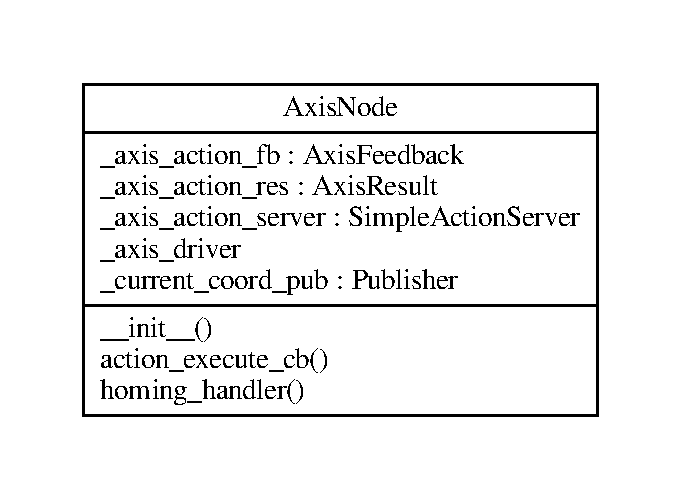
\includegraphics{images/UML/axis_driver/axis_node.pdf}
        \caption{UML diagram for the \texttt{AxisNode} class.}
        \label{fig:axis_uml_node}
    \end{subfigure}%
\end{figure}
\begin{figure}[H]
    \ContinuedFloat
    \centering
    % UML: AxisDriver
    \begin{subfigure}{\textwidth}
        \centering
        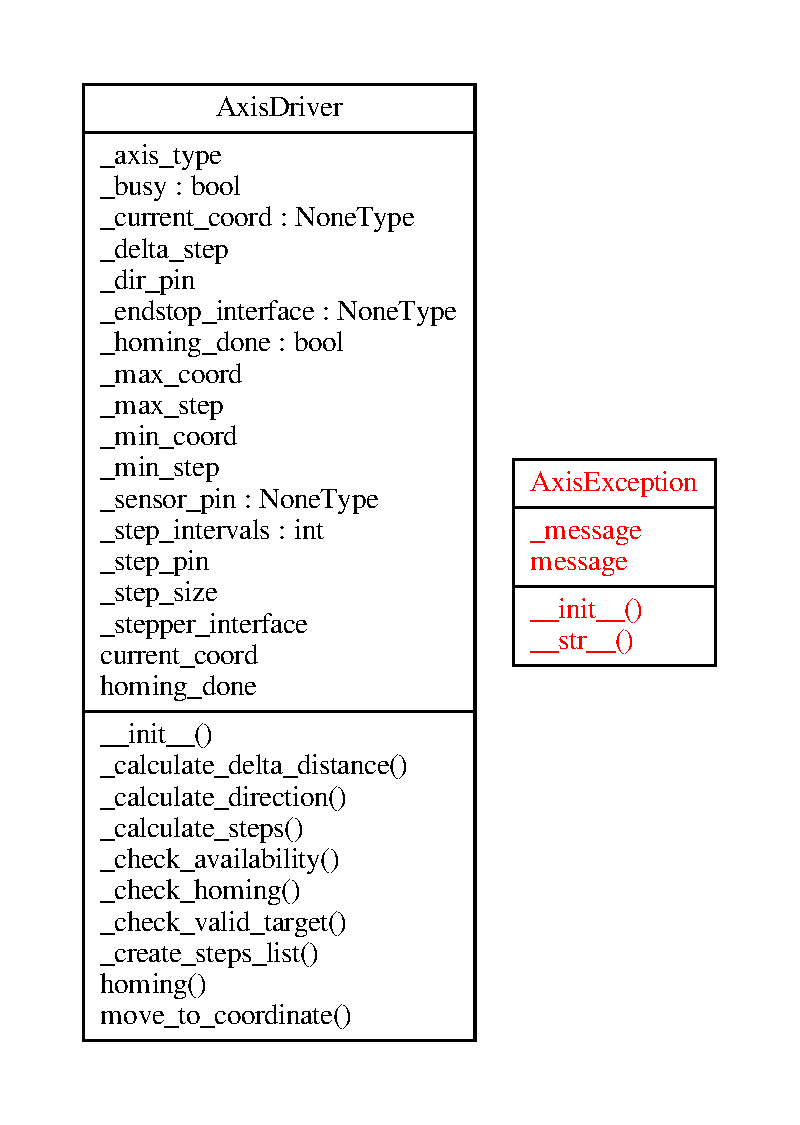
\includegraphics{images/UML/axis_driver/axis_driver.pdf}
        \caption{UML diagram for the \texttt{AxisDriver} class.}
        \label{fig:axis_uml_driver}
    \end{subfigure}%
\end{figure}
\begin{figure}[H]
    \ContinuedFloat
    % UML: StepperInterface
    \begin{subfigure}{0.5\textwidth}
        \centering
        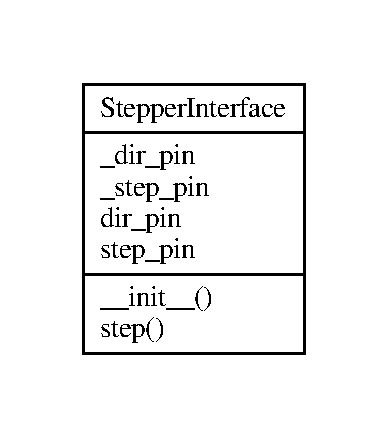
\includegraphics{images/UML/axis_driver/stepper_interface.pdf}
        \caption{UML diagram for the \texttt{StepperInterface} class.}
        \label{fig:axis_uml_stepper}
    \end{subfigure}
    % UML: EndstopInterface
    \begin{subfigure}{0.5\textwidth}
        \centering
        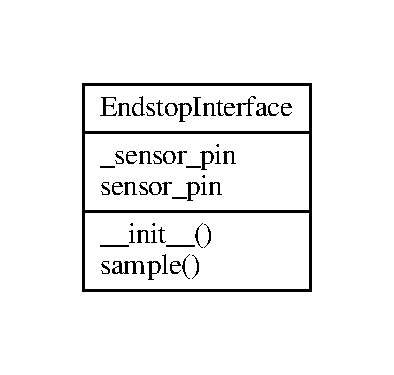
\includegraphics{images/UML/axis_driver/endstop_interface.pdf}
        \caption{UML diagram for the \texttt{EnstopInterface} class.}
        \label{fig:axis_uml_endstop}
    \end{subfigure}
    \caption{UML diagrams for the axis driver software utility.}
    \label{fig:axis_uml}
\end{figure}

The GPR-20 robot axis is intended to be used under the ROS framework even if the driver itself (\texttt{AxisDriver}) can work independently from the ROS interface. The ROS architecture for the GPR-20 axis driver is shown on figure \ref{fig:axis_ros_graph}. The ROS interface for the axis driver makes use of topics, services, actions and parameters. Parameters are used to setup the driver and define its behavior and are specified on table \ref{tab:axis_ros_params}. The axis driver ROS interface provides a single service: \texttt{homing}. The \texttt{homing} service commands the axis to execute the homing sequence to allow further movement. A single topic is also available and consists of the \texttt{current\_coord}. This topic publishes the axis current coordinate continuously. Finally, the ROS interface provides an action to move the axis. The action receives a goal and publishes the result depending on the execution status. There is no feedback from the action since the \texttt{current\_coord} publishes the same information.

\begin{table}[H]
    \centering
    \begin{tabular}{|c|p{10cm}|}
        \hline
        \textbf{Parameter} & \multicolumn{1}{c|}{\textbf{Description}} \\ \hline
        \texttt{dir\_pin} & Pin number for the direction input of the stepper motor driver. \\ \hline
        \texttt{step\_pin} & Pin number for the step input of the stepper motor driver. \\ \hline
        \texttt{sensor\_pin} & Pin number for the sensor pin input. Not required for rotational axes. \\ \hline
        \texttt{step\_size} & Step size for axis. Consists of the minimum coordinate change made by a step from the motor. \\ \hline
        \texttt{min\_step} & Minimum pause value for a step in seconds. Defines the maximum speed of the axis movement. \\ \hline
        \texttt{max\_step} & Maximum pause value for a step in seconds. Defines the minimum speed of the axis movement. \\ \hline
        \texttt{delta\_step} & Step pause value minimum change in seconds. Used to define how many different speed values are available for the axis. \\ \hline
        \texttt{min\_coord} & Minimum coordinate value for axis. Defines the lower bound for the axis. It is also the initial value for the axis current coordinate. \\ \hline
        \texttt{max\_coord} & Maximum coordinate value for axis. Defines the upper bound for the axis. \\ \hline
        \texttt{type} & Axis type. Can be either linear (`LIN') or rotational (`ROT'). \\ \hline
    \end{tabular}
    \caption{GPR-20 Axis Driver ROS parameters definition.}
    \label{tab:axis_ros_params}
\end{table}

\begin{figure}[H]
    \centering
    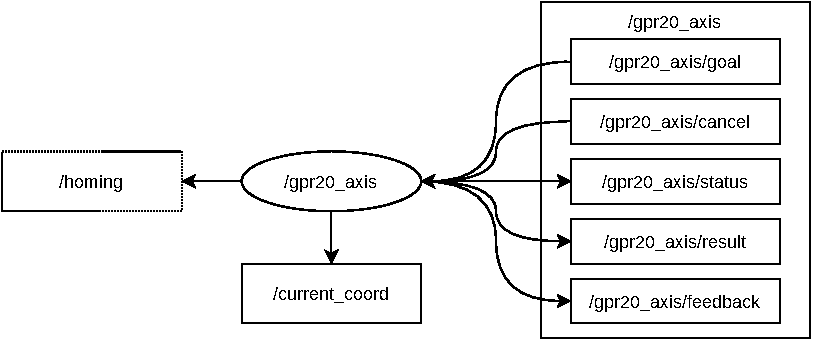
\includegraphics{images/ROS/axis_driver/ros_axis_driver.pdf}
    \caption{ROS graph diagram for the axis driver utility.}
    \label{fig:axis_ros_graph}
\end{figure}

\subsection{Height Sensor}
The GPR-20 height sensor driver utility is responsible of acquiring distance measurements from the antennae mount sensor. Two abstraction levels are defined for the sensor driver: high and mid. The abstraction layers features are shown on table \ref{tab:height_abstraction}. There is no low abstraction level since it would correspond to reading the analog-digital converter which is implemented in an open-source library. The mid abstraction level handles the sensor reading using the aforementioned library and the conversion to a distance value. Finally, the high abstraction level defines the ROS interface for the utility.

\begin{table}[H]
    \centering
    \begin{tabular}{|c|p{10cm}|}
        \hline
        \textbf{Abstraction Level} & \multicolumn{1}{c|}{\textbf{Features}} \\ \hline
        High & - Makes use of the sensor driver class to acquire distance data. \newline - Includes the ROS interface for the height sensor. \\ \hline
        Mid & - Instances the analog/digital converter library. \newline - Converts the sensor data into a distance value. \\ \hline
    \end{tabular}
    \caption{Abstraction levels for the axis driver utility.}
    \label{tab:height_abstraction}
\end{table}

The two defined abstraction layer are mapped to Python classes that implement the features described on table \ref{tab:height_abstraction}. The mid abstraction layer is mapped to \texttt{HeightDriver} and implements a single public method that takes the distance measurement. The \texttt{HeightDriver} class makes use of the \texttt{MCP3008} library to read the MCP3008 analog/digital converter through the Raspberry Pi's SPI interface. Once the MCP3008 data is read, it is converted to a distance value using a formula derived from the sensor datasheet. The high abstraction level is mapped to the \texttt{HeightNode} class that implements the ROS interface for the height utility. A service is implemented in the \texttt{HeightNode} in order to provide the distance measurement using the ROS interface. The distance measurement is sent in the response for the \texttt{get\_height} service. UML diagrams for the \texttt{HeightDriver} and \texttt{HeightNode} classes are shown on figures \ref{fig:height_uml_driver} and \ref{fig:height_uml_node}. A graph diagram for the height sensor utility is shown on figure \ref{fig:height_graph}.

\begin{figure}[H]
    % UML: HeightDriver
    \begin{subfigure}{0.5\textwidth}
        \centering
        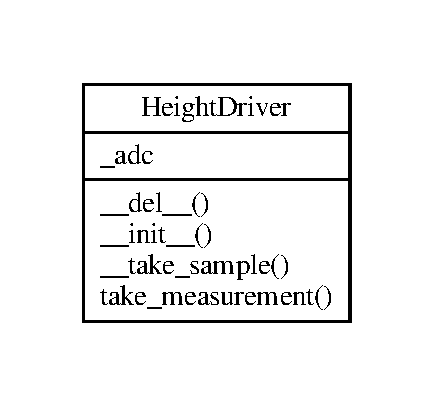
\includegraphics{images/UML/height_sensor/height_driver.pdf}
        \caption{UML diagram for the \texttt{HeightDriver} class.}
        \label{fig:height_uml_driver}
    \end{subfigure}
    % UML: HeightNode
    \begin{subfigure}{0.5\textwidth}
        \centering
        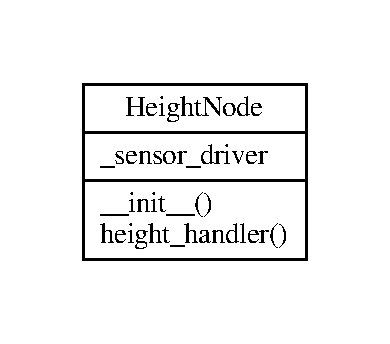
\includegraphics{images/UML/height_sensor/height_node.pdf}
        \caption{UML diagram for the \texttt{HeightNode} class.}
        \label{fig:height_uml_node}
    \end{subfigure}
    \caption{UML diagrams for the height sensor utility.}
    \label{fig:height_uml}
\end{figure}

\begin{figure}[H]
    \centering
    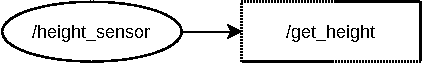
\includegraphics{images/ROS/height_sensor/ros_height_sensor.pdf}
    \caption{ROS graph diagram for the height sensor utility.}
    \label{fig:height_graph}
\end{figure}

\subsection{VNA Acquisition}
The VNA acquisition utility is responsible of acquiring the VNA data from the device and make it available to the software architecture. Two abstraction levels are defined for the VNA acquisition utility: high and mid. The mid abstraction level corresponds to a driver that implements code to configure the VNA connection, frequency sweep parameters and get both frequency and trace data. The ROS interface for the utility is implemented in the \texttt{VNANode} class and define the service servers for the utility features. Table \ref{tab:acquisition_abstraction} presents the abstraction levels for the VNA acquisition utility.

\begin{table}[H]
    \centering
    \begin{tabular}{|c|p{10cm}|}
        \hline
        \textbf{Abstraction Level} & \multicolumn{1}{c|}{\textbf{Features}} \\ \hline
        High & - Provide four services to configure and acquire data from the VNA. \newline - Instantiates the VNA driver class to execute the requested procedures. \\ \hline
        Mid & - Uses the \texttt{vxi11} library to communicate with the VNA device. \newline - Defines the processes required to connect/disconnect from the device, configure its parameters and request data. \\ \hline
    \end{tabular}
    \caption{Abstraction levels for the VNA acquisition utility.}
    \label{tab:acquisition_abstraction}
\end{table}

The abstraction levels presented in table \ref{tab:acquisition_abstraction} are implemented in two classes. The \texttt{VNADriver} is the implementation for the mid abstraction level and \texttt{VNANode} for the high abstraction level. UML diagrams for \texttt{VNADriver} and \texttt{VNANode} are presented in figures \ref{fig:acquisition_uml_driver} and \ref{fig:acquisition_uml_node}. The \texttt{VNADriver} class communicates with the VNA device under the VXI11 protocol and uses the \texttt{vxi11} library to execute do so. The \texttt{VNANode} provide four service servers whose handlers call the respective methods from the driver implementation. The services are used for connecting and disconnecting the device, configure the frequency sweep parameters (start and stop frequencies and number of points), get the frequencies vector and get a trace. Figure \ref{fig:acquisition_graph} presents the graph diagram for the \texttt{vna\_acquisition} node.

\begin{figure}[H]
    % UML: VNADriver
    \begin{subfigure}{0.5\textwidth}
        \centering
        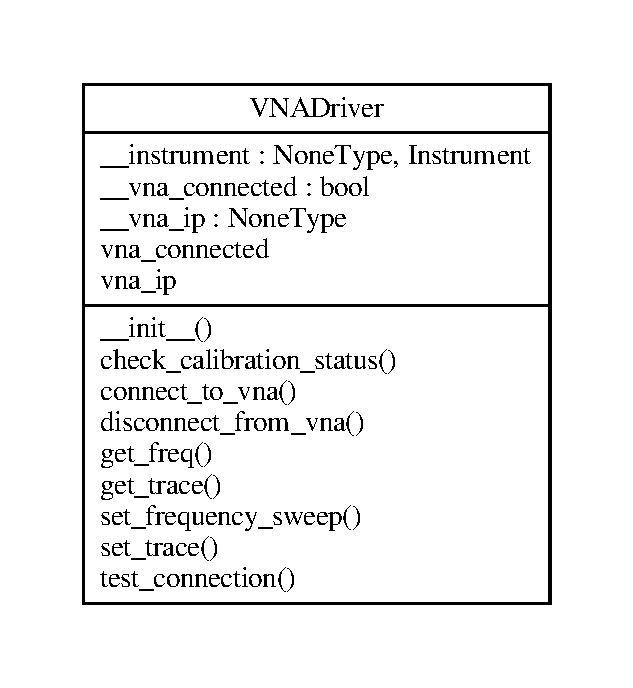
\includegraphics{images/UML/vna_acquisition/vna_driver.pdf}
        \caption{UML diagram for the \texttt{VNADriver} class.}
        \label{fig:acquisition_uml_driver}
    \end{subfigure}
    % UML: VNANode
    \begin{subfigure}{0.5\textwidth}
        \centering
        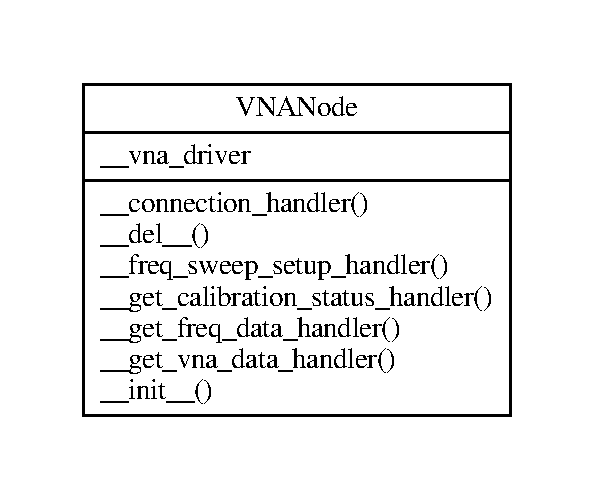
\includegraphics{images/UML/vna_acquisition/vna_node.pdf}
        \caption{UML diagram for the \texttt{VNANode} class.}
        \label{fig:acquisition_uml_node}
    \end{subfigure}
    \caption{UML diagrams for the height sensor utility.}
    \label{fig:acquisition_uml}
\end{figure}

\begin{figure}[H]
    \centering
    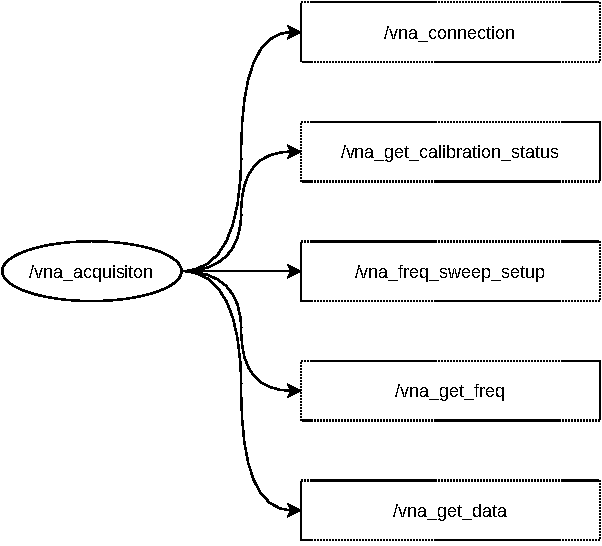
\includegraphics{images/ROS/vna_acquisition/ros_vna_acquisition.pdf}
    \caption{ROS graph diagram for the height sensor utility.}
    \label{fig:acquisition_graph}
\end{figure}

\subsection{Data Processing}
The Data Processing is the utility that stores the robot data in a persistent storage. The data processing utility receives the data from the ROS communication mechanisms and then stores it. Since data storage can be a time-consuming process, threads are used to avoid blocking the utility when multiple storage requests are received. It must be noted that the processing time depends on the used storage technology. Data is stored using the JSON format and includes information regarding the coordinates and date in which data was acquired, the height sensor data and the VNA trace. Three abstraction levels are defined for the Data Processing utility: high, mid and low. The high abstraction level is used to integrate the ROS functionality of the utility i.e. the service in which data is received. The mid abstraction level provides the mechanisms to execute the storage threads. Finally, the low level functionality consist of the processing stages for the data. Table \ref{tab:processing_abstraction} presents the abstraction levels of the Data Processing utility.

\begin{table}[H]
    \centering
    \begin{tabular}{|c|p{10cm}|}
        \hline
        \textbf{Abstraction Level} & \multicolumn{1}{c|}{\textbf{Features}} \\ \hline
        High & - Provide a single service in which a request to storage data is received. \newline - Instantiates the main processing class to execute the storage procedure. \\ \hline
        Mid & - Executes the processing stages for the data from parsing to storage. \\ \hline
        Low & - Defines the procedures for data processing. \newline - Data does not solely consists of VNA traces, it also includes the sample coordinates, antennae height, timestamp and unique identifiers. \\ \hline
    \end{tabular}
    \caption{Abstraction levels for the data processing utility.}
    \label{tab:processing_abstraction}
\end{table}

The VNA processing utility is implemented in three classes: the \texttt{ProcessingNode} class for the high abstraction level, the \texttt{DataProcessing} class for the mid abstraction level and the \texttt{StorageThread} for the low abstraction level. The \texttt{ProcessingNode} class implements a single method to handle the storage request received via the \texttt{/store\_data} service. The high-level class also instantiates the \texttt{DataProcessing} class. This class implements a single method that bypasses the data to the low-level thread. This approach is used to facilitate the inclusion of different processing stages for the VNA data. Finally, the \texttt{StorageThread} parses the data into the JSON format and stores the data.  

\subsection{Main Control}
The main control is the utility that coordinates the features provided by the remaining utilities from the software architecture. The user configures the main control through the user interface in order to use the GPR-20 robot. Configuring the control unit is usually done from the user interface yet it can be configured from other interfaces such as command consoles and web applications. 

The main control interfaces with the user through services and topics of two different types: configuration and feedback. Configuration interface corresponds to the mechanisms in which the survey parameters and commands are passed to the control. Feedback interfaces provides data from the control unit to the user. Feedback data is intended to be displayed on the user interface. Table \ref{tab:control_user_comm} presents the ROS communication mechanism for the main control unit. The \texttt{set\_survey\_parameters}, \texttt{start\_survey} and \texttt{stop\_survey} correspond to the configuration mechanisms. In the other hand, \texttt{control\_status}, \texttt{control\_target\_coordinate}, \texttt{control\_current\_coordinate} and \texttt{control\_survey\_data} correspond to the feedback mechanisms.

\begin{singlespace}
    \begin{xltabular}{\textwidth}{|p{5cm}|l|X|}
    
        \hline \textbf{Name} & \textbf{Mechanism} & \textbf{Description} \\ \hline
        \endhead
        
        \hline \textbf{Name} & \textbf{Mechanism} & \textbf{Description} \\ \hline
        \endfirsthead
        
        \multicolumn{3}{|c|}{\textit{Continues on next page.}}
        \endfoot
        
        \caption{Communication mechanism between the GPR-20 main control and the user interface.} \label{tab:control_user_comm}
        \endlastfoot
        
        \texttt{set\_survey\_parameters} & Service & This service is sent by the user with the survey parameters. Survey parameters include the frequency start and stop frequencies, the sampled frequency points, start and stop values for both the X and Y axes, and the surveyed points per axis. \\ \hline
        \texttt{start\_survey} & Service & This service is used as the start command for the survey process. The service message does not carry any data in it. \\ \hline
        \texttt{stop\_survey} & Service & This service is used as the stop command for the survey process. It must be noted that this command is reserved for the situations in which the user might want to stop the surveying process. The survey stops itself when finished otherwise. \\ \hline
        \texttt{control\_status} & Topic & This topic broadcasts the general status of the GPR-20 robot software. The topic message contains a status code and a status message. \\ \hline
        \texttt{control\_target\_coordinate} & Topic & This topic publishes the current target coordinate of the GPR-20 positioner. The topic message contains the three relevant coordinates of the GPR-20 robot. A negative value is used when no survey is taking place. \\ \hline
        \texttt{control\_current\_coordinate} & Topic & This topic publishes the condensed current coordinate of the GPR-20 robot. \\ \hline
        \texttt{control\_survey\_data} & Topic & This topic publishes statistical data of the current survey. This data includes the completion percentage, total points, and visited points. \\ \hline
    \end{xltabular}
\end{singlespace}

Additional communication mechanism are defined in order to command and exchange data between the main control and the different utilities. These communication allows the main control to effectively execute the required commands. The main control directly commands three (3) \texttt{Axis Driver} instances, the \texttt{Height Sensor} utility, the \texttt{VNA Acquisition} utility, and the \texttt{VNA Processing} utility. Table \ref{tab:control_software_comm} presents the communication mechanisms between the main control and the different software utilities. It must be noted that since three (3) \texttt{Axis Driver} instances are used with the same interface, their communication mechanisms are presented only once.

\begin{singlespace}
    \begin{xltabular}{\textwidth}{|p{5cm}|l|l|X|}
    
        \hline \textbf{Name} & \textbf{Utility} & \textbf{Mechanism} & \textbf{Description} \\ \hline
        \endhead
        
        \hline \textbf{Name} & \textbf{Utility} & \textbf{Mechanism} & \textbf{Description} \\ \hline
        \endfirsthead
        
        \multicolumn{4}{|c|}{\textit{Continues on next page.}} \\ \hline
        \endfoot
        
        \caption{Communication mechanism between the GPR-20 main control and the software utilities.} \label{tab:control_software_comm}
        \endlastfoot
        
        \texttt{axis} & \texttt{Axis Driver} & Action & This action provides the mechanism to set the target coordinate of the axis and execute the required movement. The action does not provide feedback since there is a topic used for this purpose. \\ \hline
        \texttt{current\_coord} & \texttt{Axis Driver} & Topic & The topic publishes the current coordinate of the axis. An specific Boolean flag is also included in the message to indicate when the axis has not executed the homing sequence. \\ \hline
        \texttt{homing} & \texttt{Axis Driver} & Service & Used to command an axis to execute the homing sequence of the driver. No response is expected from this service besides from changing the homing status flag. \\ \hline
        \texttt{get\_height} & \texttt{Height Sensor} & Service & This services provides the requester with the latest measurement from the height sensor. Using the service allows to synchronize the height measurement with the data acquisition process. \\ \hline
        \texttt{measured\_height} & \texttt{Height Sensor} & Topic & The topic continuously streams the measurement from the height sensor. This information is used for feedback purposes. \\ \hline
        \texttt{get\_data} & \texttt{VNA Acquisition} & Service & It is used to retrieve the data from the VNA instrument. The data corresponds to the S21 parameter acquired within the specified bandwidth. \\ \hline
        \texttt{get\_freq} & \texttt{VNA Acquisition} & Service & This service is used to retrieve the frequency values in which data is acquired. This service is used to determine which frequencies are sampled during the data acquisition process. \\ \hline
        \texttt{connection} & \texttt{VNA Acquisition} & Service & This communication mechanism is used to execute the VNA connection in the \texttt{VNA Acquisition} node. The response consists of a Boolean flag indicating the result of the connection procedure. \\ \hline 
        \texttt{freq\_sweep\_setup} & \texttt{VNA Acquisition} & Service & This service is used to configure the VNA device with the frequency sweep parameters. \\ \hline
        \texttt{store\_data} & \texttt{VNA Processing} & Service & It is used to store data in a persistent location. Data does not only include the VNA responses but its coordinates, height measurement and frequency values. \\ \hline
    \end{xltabular}
\end{singlespace}

The main control utility is implemented in four (4) classes along three abstraction levels. The used abstraction levels do not correspond to the defined abstraction levels for other utilities. In turn, the abstraction levels are defined to properly interface with the different software utilities. Table \ref{tab:control_abstraction} presents the three abstraction levels of the main control software utility. 

\begin{singlespace}
    \begin{xltabular}{\textwidth}{|l|X|}
    
        \hline \textbf{Abstraction Level} & \textbf{Description} \\ \hline
        \endhead
    
        \caption{Abstraction levels for the main control.} \label{tab:control_abstraction}
        \endlastfoot
        
        \hline \multicolumn{2}{|c|}{\textit{Continues on next page.}} \\ \hline
        \endfoot
        
        High & The high abstraction level is reserved for the communication between the graphical user interface and the main control. This abstraction level can either receive or send information and/or commands from the control to the interface and vice versa. This is defined as the highest level as the information and commands are closer to the user. \\ \hline
        Mid & This abstraction level organizes and commands the different actions in the robot in order to execute them as intended. The mid abstraction level implements the functionalities and code to execute the survey keeping into account the synchronization between the different actions. It must be noted that this abstraction level does not communicates directly with other software utilities. \\ \hline
        Low & This abstraction level groups the functionalities to be accessed in different utilities. The idea of the low abstraction level is to implement the communication mechanisms between the control and other utilities. \\ \hline
    \end{xltabular}
\end{singlespace}


\subsection{User Interface}
The user interface is the utility that provides the user with a graphical interface from which the robot can be commanded. The graphical interface is connected to ROS in order to send and receive both data and commands. The graphical interface is built using the PyQt5 framework. The graphical interface provides an user to execute the functionalities described on table \ref{tab:user_interface}.

\begin{table}[h]
    \centering
    \begin{tabular}{|p{5cm}|p{10cm}|}
        \hline \textbf{Functionality} & \textbf{Description} \\ \hline
        Input the VNA IP address &  The VNA IP is used to connect the VNA acquisition utility with the device itself. It must be manually entered by the user based on the device configuration. \\ \hline
        Input the VNA frequency points & The number of frequency points that will be sampled depend on the VNA calibration. Timing constrains and data quality also are taken into account to define the frequency points. \\ \hline
        Input the VNA start/stop frequencies & The start/stop frequencies of the VNA sampling are defined by the user based on data quality. The frequencies are also defined based on the VNA calibration. \\ \hline
        Input the sample start/stop coordinates & The start/stop coordinates will determine how large will be the survey area. The coordinates are referred to the linear axes of the GPR-20 robot. Each coordinate consists of a pair of values that range from 0 to 800. There is no constrain on which value (start or stop) needs to be higher than the other thus a \textit{reverse} survey can be performed. \\ \hline
        Input the sample points per axis & The number of sample points define the resolution in which data will be acquired. The user will input a number that defines the number of points in which the axis will stop considering the whole length of the axis. \\ \hline
        Start/stop a data-acquisition & The user is able to either start and stop the data-acquisition via the user interface. If an error is raised when starting the data-acquisition, a pop-up will show the error. The start and stop buttons will be enabled or disabled based on the data-acquisition status. \\ \hline
    \end{tabular}
    \caption{User interface functionalities.}
    \label{tab:user_interface}
\end{table}

The functionalities are implemented in such a way that the user modifies the data in the interface and sends the commands to the main control. The decoupling that exists between the user interface and the main control allows for some situations to arise and compromise the user experience. These situations consists of the main control being at certain state with the user interface not appropriately representing it. For example, the main control could be executing a data-acquisition survey while the interface allows for sending parameters and the start command. Two workarounds were implemented for this situations: providing a bidirectional communication between the user interface and the main control, and assigning responsibilities to the user interface.

The bidirectional communication between the user interface and the main control is critical for a consistent user experience. The main control provides the user interface with feedback in order to prevent congruent situations to arise. The user interface then changes its status to only allow for valid actions to take place. Following with the previous example, if the user interface is initialized after a survey is initialized, the main control provides feedback to the user interface in order to prevent sending new parameter values and/or the start survey command. This prevention is done by locking or unlocking the user interface input fields. It must be noted that although the user interface prevents such situations from happening, the main control can handle such erroneous requests without compromising the data acquisition process. 

The second workaround makes the user interface is responsible on checking the validity of the input data from the user. Checking the validity does not check that values are correct but that they can be properly used to configure the robot. For example, the user can input the VNA IP address with only three out of the four fields with a number. In this situation, the user interface will check that the IP address is valid thus warning the user that its value should be checked. However, checking that the entered IP address correspond to the VNA address is done in the main control. In this situation, the user interface will receive the feedback from the main control and then warn the user on the erroneous data. Table \ref{tab:gui_checks} presents the input fields for the user interface with the checks that are performed in the user interface.

\begin{singlespace}
    \begin{xltabular}{\textwidth}{|l|X|}
    
        \hline \textbf{Field} & \textbf{Checks} \\ \hline
        \endhead
        
        \caption{Validity checks executed on the user interface.} \label{tab:gui_checks}
        \endlastfoot

        VNA IP Address & - Check that it has its four numbers set. \\ \hline
        Start Frequency & - Check that is a value different from zero. \newline - Check that the value is lower than the stop frequency. \\ \hline
        Stop Frequency & - Check that is a value different from zero. \newline - Check that the value is higher than the start frequency. \\ \hline
        Frequency Points & - Check that is a value different from zero. \newline - Check that the value is lower or equal than four thousand (4000). \\ \hline
        X-Axis Start Coordinate & - Check that the value is positive. \newline - Check that the value is lower than eight hundred (800). \\ \hline
        X-Axis Stop Coordinate & - Check that the value is positive. \newline - Check that the value is lower than eight hundred (800). \\ \hline
        X-Axis Points & - Check that the value is greater than two (2). \\ \hline
        Y-Axis Start Coordinate & - Check that the value is positive. \newline - Check that the value is lower than eight hundred (800). \\ \hline
        Y-Axis Stop Coordinate & - Check that the value is positive. \newline - Check that the value is lower than eight hundred (800). \\ \hline
        Y-Axis Points & - Check that the value is greater than two (2). \\ \hline
    \end{xltabular}
\end{singlespace}

The user interface is presented in figures \ref{fig:ui_img_control} and \ref{fig:ui_img_status}. The user interface allow the user to input the VNA IP address, the frequency parameters and the coordinate parameters. The VNA address is entered via four input fields. This separation is done since the user interface is designed for a touchscreen where a keyboard might not be present. The remaining input fields receive the input values from the user via the up and down arrows. The arrows allow for value changes in steps. The value of the steps is configured by the user in order to allow for value changes more rapidly.

\begin{figure}[h]
    \centering
    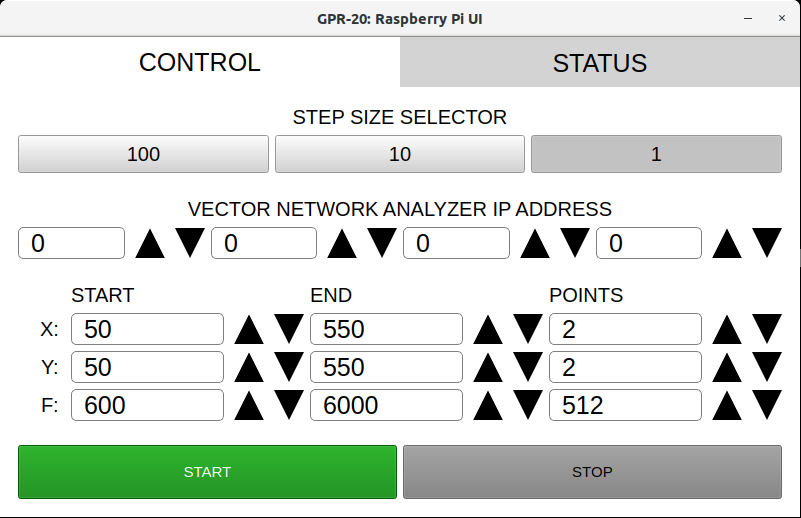
\includegraphics[width=0.6\textwidth]{images/software/UI_control.png}
    \caption{User interface (control) for the GPR-20 robot.}
    \label{fig:ui_img_control}
\end{figure}

\begin{figure}[h]
    \centering
    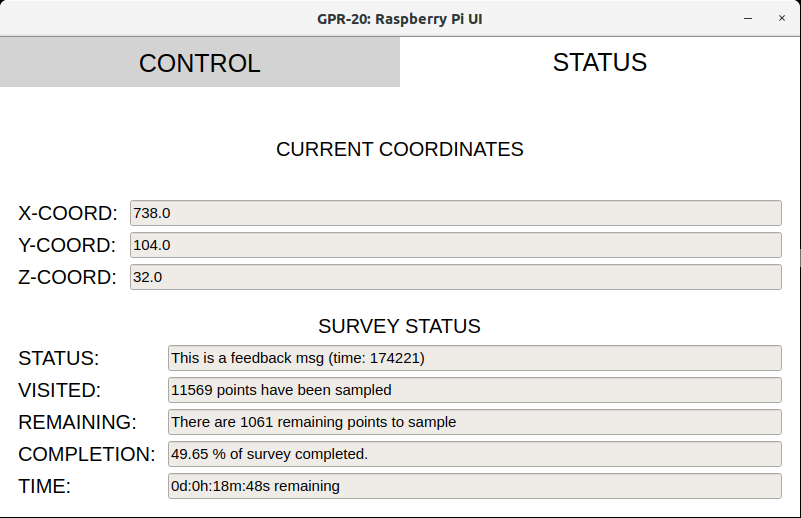
\includegraphics[width=0.6\textwidth]{images/software/UI_status.png}
    \caption{User interface (status) for the GPR-20 robot.}
    \label{fig:ui_img_status}
\end{figure}

\end{document}
